\documentclass[../main.tex]{subfiles}
\begin{document}
\chapter{The double-$\tau_h$ + jet trigger}
\label{hh:chapter:trigger}

In view of Run 3, a lot of effort has been dedicated in order to maximize the collection efficiency from physics processes such as H~$\to\tau\tau$ and HH~$\to$~bb$\tau\tau$. In these two cases, in most events the produced $\tau\tau$ pair is accompanied by one or more jets coming from the hard-scattering processes or from QCD radiation (in addition to the 2 b-jets coming from the other H in the HH~$\to$~bb$\tau\tau$ process), as seen in Fig.~\ref{hh:fig:trig_ngenjets}.

In both \htt{} and \hhbbtt{} analyses, the trigger strategy during Run-1 and Run-2 for the \tauh\tauh{} channel consisted in a double-$\tau_h$ selection, with a $p_T$ threshold of 32 and 35~GeV at L1 and HLT level, respectively, during 2018 data-taking. By including in the menu a new trigger that requires two $\tau_h$ and an additional jet (whose $p_T$ spectrum at L1 is shown in Fig.~\ref{hh:fig:trig_l1jet_pt}), the $p_T$ threshold on the $\tau_h$ could be lowered. By doing so, as more $\tau_h$ will be available for triggering (see Fig.~\ref{hh:fig:trig_l1tau_pt}), the acceptance of both analyses could be enlarged.


\begin{figure}[h!]
\begin{center}
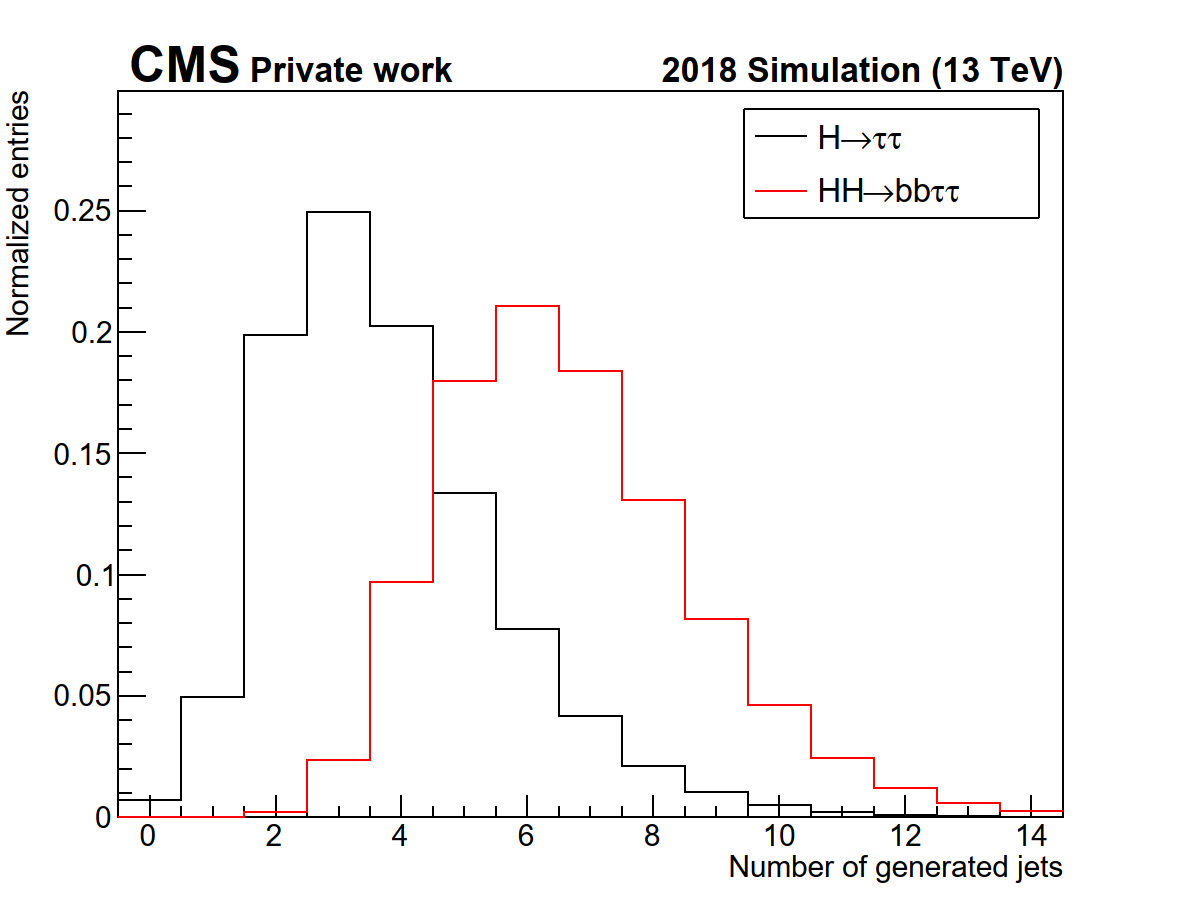
\includegraphics[width=0.6\textwidth]{Images/ngenjets}
\end{center}
\caption[Number of jets at generator level]{Total number of jets per event at generator level for H~$\to\tau\tau$ (black) and HH~$\to$~bb$\tau\tau$ (red) processes, both produced via ggF.}
\label{hh:fig:trig_ngenjets}
\end{figure}

\begin{figure}[h!]
\begin{center}
\includegraphics[width=0.5\textwidth]{Images/leading_jet_pt}
\end{center}
\caption[L1 leading jet $p_T$]{L1 leading jet $p_T$ for the H~$\to\tau\tau$ (black) and HH~$\to$~bb$\tau\tau$ (red) processes, both produced via ggF.}
\label{hh:fig:trig_l1jet_pt}
\end{figure}

\begin{figure}[h!]
\begin{center}
\subfloat{\includegraphics[width=0.5\textwidth]{Images/l1tau_pt_htt_ggf_new}}
\subfloat{\includegraphics[width=0.5\textwidth]{Images/l1tau_pt_hhbbtt_ggf_new}}
\end{center}
\caption[L1 $\tau_h$ $p_T$]{L1 leading and subleading $\tau_h$ $p_T$ for the H~$\to\tau\tau$ (left) and HH~$\to$~bb$\tau\tau$ (right) processes, both produced via ggF. In both cases, below the double-$\tau_h$ trigger $p_T$ threshold (32~GeV in 2018), many $\tau_h$ would be available for triggering.}
\label{hh:fig:trig_l1tau_pt}
\end{figure}

The following sections discuss the design and performance of a new L1 seed with two $\tau_h$ and one jet to be included in the L1 Menu and a new HLT path seeded by this new L1 seed. The goal is that the newly defined L1 seed and HLT path add as little rate as possible but increase the final acceptance on the \htt{} and \hhbbtt{} analyses. The acceptance increase at trigger level is enhanced by the possibility of loosening correspondingly the offline selection cuts. In the \htt{} analysis \cite{hh:htt_run2}, the two $\tau_h$ are selected if their $p_T > 40$~GeV, while the selection on the jets is different in the four categories defined. In this study, only two categories are considered, obtained as a simplification of the most sensitive analysis categories: the 1-jet, high $p_T$ category, where we consider events with one jet with $p_T > 70$~GeV; and the 2-jet category, where we select events with at least two jets with $p_T > 30$~GeV. In the \hhbbtt{} analysis, as was described in Chapter~\ref{hh:chapter:analysis}, events with at least two $\tau_h$ with $p_T>40$~GeV and at least two jet candidates with $p_T>20$~GeV are selected.

The goal of this study was to include the new trigger seed and path in the menus devoted to collisions during 2022, where an average PU of 53 and 2748 bunches per beam were expected. The design and optimization of the triggers, however, will consider samples from 2018, which will be adapted to the expected 2022 conditions. To estimate the rate added by the new trigger, zero bias samples will be considered. These samples are characterised by being unbiased by the trigger decision, as they only require the crossing of two bunches.

Section~\ref{hh:sec:l1seeds} describes the optimization procedure followed to include the L1 double-\tauh{}+jet seed. Section~\ref{hh:sec:l1_performance} shows the performance results of the new L1 seed obtained from Run 3 data and simulated samples. Section~\ref{hh:sec:hlt_doubletaujet} describes the HLT double-\tauh{}+jet path included in the menu, and its performance is evaluated in Section~\ref{hh:sec:hlt_performance}.

The development of this new trigger was a substantial part of my thesis, from the inclusion of the new L1 seed after a long optimization period, to the development of the corresponding HLT path. I am the main responsible for the performance studies from both L1 seed and HLT path and the first studies on the sensitivity gained thanks to this new trigger in a future Run 3 \hhbbtt{} analysis.




\section{The L1 double-$\tau_h$ + jet trigger}
\label{hh:sec:l1seeds}

In the L1 menu used during the Run-2 data taking, the only seeds that consider hadronic $\tau$ decays were the \texttt{L1\_DoubleIsoTauXer2p1} seeds, where two isolated $\tau_h$ with $p_T\geq X$~GeV and $|\eta|<2.1$ are selected. The threshold $X$ varied during the data-taking, with a value of $X=32~$GeV during 2018. The strategy followed in this study is to include a new seed in the L1 Menu with two isolated $\tau_h$ objects and one jet object identified by the $\mu$GT. This new seed complements the already present double-$\tau_h$ seed with the same 32~GeV threshold (or with a larger $p_T$ threshold in order to keep the rate as low as possible). A particular treatment has to be given to seeds involving $\tau_h$ and jet objects simultaneously, as both, $\tau_h$ and jets, are reconstructed as purely calorimetric objects. Therefore, all $\tau_h$ objects enter the L1 jet collection, and some of the L1 jets also appear in the L1 $\tau_h$ collection. This effect is illustrated in Fig.~\ref{hh:fig:l1_tau_jet_dR}, where the minimal $\Delta R$ between all L1 $\tau_h$'s and jets is computed. At small values of $\Delta R$ a peak is observed, coming from the overlap between the L1 $\tau_h$ and jet collections. To reduce this effect, only L1 jets that are separated more than $\Delta R>0.5$ with the selected $\tau_h$ are considered. This operation is called overlap removal \cite{intro:l1_13tev}. It was already present in the $\mu$GT before the inclusion of the new seed, both in the firmware and its software emulator. However, while including the new seed, some discrepancies arose between both implementations, so the $\mu$GT software emulator had to be was modified accordingly.

\begin{figure}[h!]
\begin{center}
\includegraphics[width=0.5\textwidth]{Images/l1_tau_jet_dR}
\end{center}
\caption[Minimal $\Delta R$ between all L1 $\tau_h$'s and jets per event]{Minimal $\Delta R$ between all L1 $\tau_h$'s and jets per event in a \htt{} ggF simulated sample. The peak at small $\Delta R$ values is due to the overlap between the L1 $\tau_h$ and jet collections.}
\label{hh:fig:l1_tau_jet_dR}
\end{figure}

As previously stated, this new double-$\tau_h$+jet seed (encoded as \texttt{L1\_Double\-IsoTauY\-er2p1\-\_JetZ\_RmOvlp\_dR0p5}, where $Y$ and $Z$ are the $p_T$ thresholds for the $\tau_h$ and jet, respectively) does not aim to replace the present \texttt{L1\_Double\-Iso\-Tau32er2p1} seed, but to complement it. However, in order to make some rate available for the new seed, increasing the double-$\tau_h$ $p_T$ threshold to a value $X$ could be needed. The rates corresponding to different values of the double-$\tau_h$ threshold are shown in Fig.~\ref{hh:fig:trig_ditau32_rate}. After the inclusion of the new seed, the aim is to keep the total rate of both seeds as close as possible to the original rate of the \texttt{L1\_Double\-Iso\-Tau32er2p1} seed, so a target rate of $\sim17$~kHz is considered.

\begin{figure}[h!]
\begin{center}
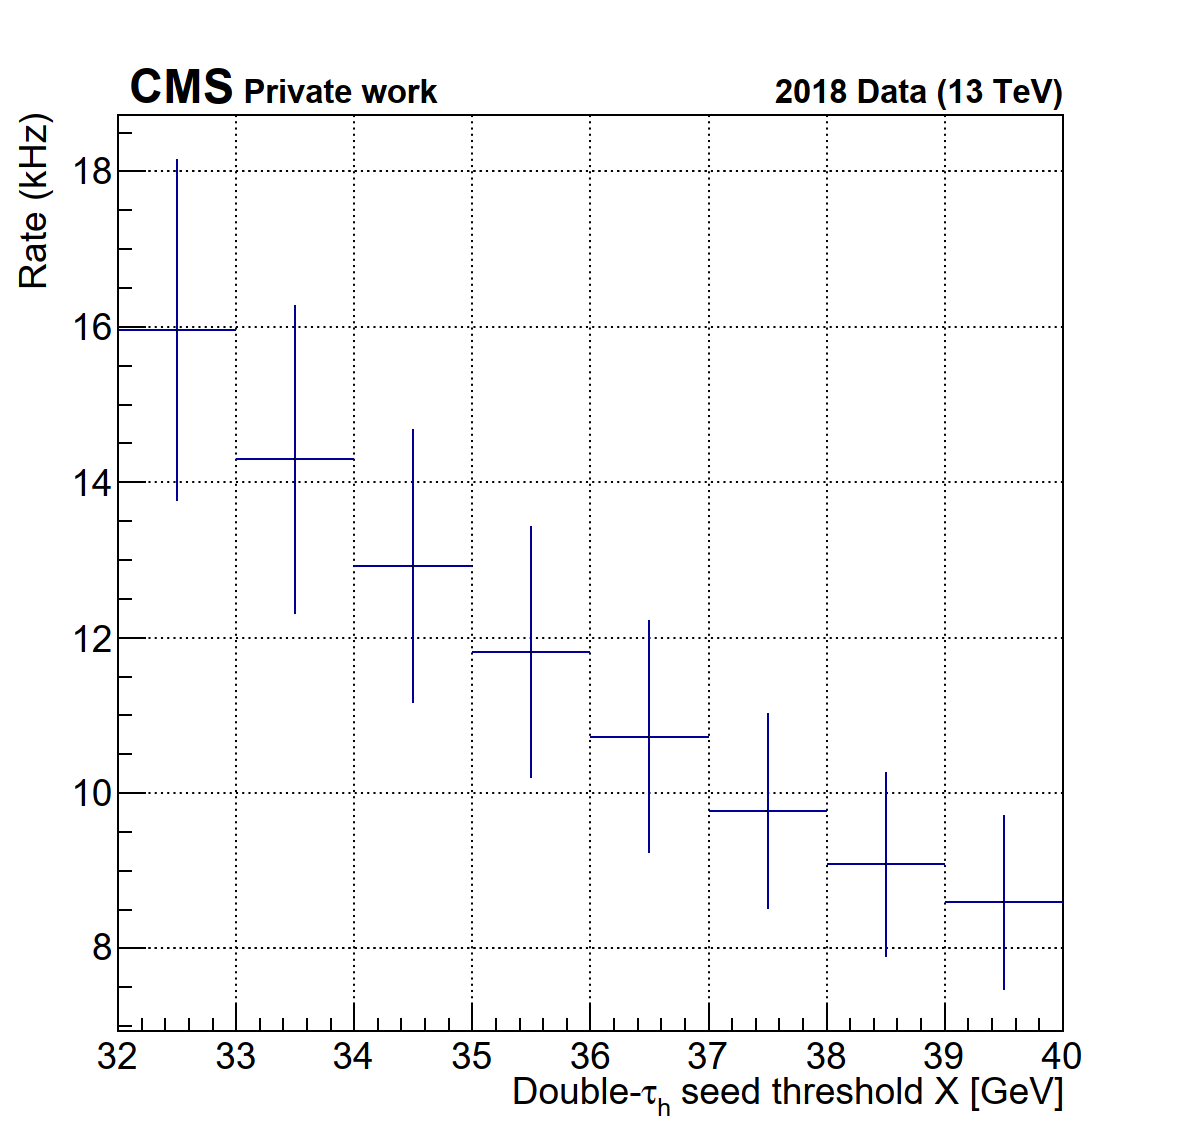
\includegraphics[width=0.5\textwidth]{Images/plot2D_ditau_sym_323755}
\end{center}
\caption[\texttt{L1\_DoubleIsoTauXer2p1} trigger seed rate]{Rate of the \texttt{L1\_DoubleIsoTauXer2p1} trigger seed under Run 3 conditions (PU 53, 2748 bunches) as a function of the $X$ threshold.}
\label{hh:fig:trig_ditau32_rate}
\end{figure}

As the aim to increase the signal acceptance, the acceptance gain when considering the two new seeds instead of the reference \texttt{L1\_Double\-IsoTau32\-er2p1} seed is computed. Four signal samples are considered, two ggF and VBF H~$\to\tau\tau$ and two ggF and VBF HH~$\to$~bb$\tau\tau$. These acceptance gains are computed not only from the L1 objects that pass the required selection cuts (grouped in the booleans \texttt{PassL1DoubleTau32}, \texttt{PassL1DoubleTauX} and \texttt{PassL1DoubleTauYJetZ}), but also applying selections to the objects obtained by the offline reconstruction that evolve accordingly to the L1 thresholds considered. In general, this evolution means that, for a given L1 $p_T$ threshold $T$, the offline threshold is obtained as $T$ + $\Delta T$. As in both target analyses the offline \tauh{} $p_T$ threshold is set to 40~GeV when using a L1 threshold of 32~GeV, a $\Delta T=8$~GeV for the $\tau_h$ is considered. For the jets, a $\Delta T=10$~GeV is taken. All $p_T$ selections for the different categories are summarised in Table~\ref{hh:tab:trig_offpt}, where one boolean associated to each seed has been defined in order to group the needed offline selections. On top of these $p_T$ cuts, all offline jets must be within $|\eta|<4.7$ and pass tight jet ID and loose PU jet ID and an overlap removal criteria with the offline $\tau_h$ ($\Delta R(\text{jet}, \tau_h)>0.5$). 

\begin{table}
	\begin{center}
	\begin{tabular}{c || c | c | c }
		                           & \multicolumn{3}{c}{Offline $p_T$ selections} \\
		                           \cline{2-4}\noalign{\vskip\doublerulesep
         \vskip-\arrayrulewidth}
         						   \cline{2-4}
		  Boolean         & \multicolumn{2}{c|}{\htt} &   \multirow{2}{*}{\hhbbtt}      \\\cline{2-3}               
		                  & 1-jet, high $p_T$ & 2-jet &  \\\hline\hline
		\texttt{PassOfflDoubleTau32} & 
			$\begin{matrix}
				p_T^{\tau_1}>40\\
				p_T^{\tau_2}>40\\
				p_T^{j_1}>70
			\end{matrix}$ &
			$\begin{matrix}
				p_T^{\tau_1}>40\\
				p_T^{\tau_2}>40\\
				p_T^{j_1}>30 \\
				p_T^{j_2}>30
			\end{matrix}$ &
			$\begin{matrix}
				p_T^{\tau_1}>40\\
				p_T^{\tau_2}>40\\
				p_T^{j_1}>20\\
				p_T^{j_2}>20
			\end{matrix}$ \\\hline
		\texttt{PassOfflDoubleTauX} & 
			$\begin{matrix}
				p_T^{\tau_1}>X+8\\
				p_T^{\tau_2}>X+8\\
				p_T^{j_1}>70
			\end{matrix}$ &
			$\begin{matrix}
				p_T^{\tau_1}>X+8\\
				p_T^{\tau_2}>X+8\\
				p_T^{j_1}>30 \\
				p_T^{j_2}>30
			\end{matrix}$ &
			$\begin{matrix}
				p_T^{\tau_1}>X+8\\
				p_T^{\tau_2}>X+8\\
				p_T^{j_1}>20\\
				p_T^{j_2}>20
			\end{matrix}$ \\\hline
		\texttt{PassOfflDoubleTauYJetZ} &
			$\begin{matrix}
				p_T^{\tau_1}>Y+8\\
				p_T^{\tau_2}>Y+8\\
				p_T^{j_1}>Z+10 \\
				p_T^{j_1}>70
			\end{matrix}$ &
			$\begin{matrix}
				p_T^{\tau_1}>Y+8\\
				p_T^{\tau_2}>Y+8\\
				p_T^{j_1}>Z+10 \\
				p_T^{j_1}>30 \\
				p_T^{j_2}>30
			\end{matrix}$ &
			$\begin{matrix}
				p_T^{\tau_1}>Y+8\\
				p_T^{\tau_2}>Y+8\\
				p_T^{j_1}>Z+10 \\
				p_T^{j_1}>20 \\
				p_T^{j_2}>20
			\end{matrix}$
	\end{tabular}
	\end{center}

	\caption[Offline $p_T$ selections associated to the L1 selections]{Offline $p_T$ selections associated to the L1 selections of \texttt{L1\_DoubleIsoTau32er2p1}, \texttt{L1\_DoubleIsoTauXer2p1} and \texttt{L1\_DoubleIsoTauYer2p1\_JetZ\_RmOvlp\_dR0p5} for the different categories, where $\tau_1$ and $\tau_2$ are the leading and subleading $\tau_h$ and $j_1$ and $j_2$ are the leading and subleading jets. All thresholds are expressed in GeV.}
	\label{hh:tab:trig_offpt}
\end{table}


Thus, the acceptance gain when adding a double-$\tau_h$+jet seed and modifying the threshold of the present double-$\tau_h$ seed can be defined as
\begin{equation}
g(X, Y, Z) = \frac{\begin{matrix}N[(\text{\texttt{PassL1DoubleTauX}} \,\,\&\&\,\, \text{\texttt{PassOfflDoubleTauX}}) \,\,||\,\, \\ \qquad\qquad\qquad(\text{\texttt{PassL1DoubleTauYJetZ}} \,\,\&\&\,\, \text{\texttt{PassOfflDoubleTauYJetZ}})] \end{matrix}}{N[\text{\texttt{PassL1DoubleTau32}} \,\,\&\&\,\, \text{\texttt{PassOfflDoubleTau32}}]}
\end{equation}
where $N$ is the number of events that pass the conditions required for given values of the $X$, $Y$ and $Z$ $p_T$ thresholds. The average acceptance gains obtained for different sets of thresholds ($X$, $Y$, $Z$) for the samples and categories considered is shown in Fig.~\ref{hh:fig:l1_trig_mean_acc}. Only the 20 sets with the highest acceptance gain in a 15-17 kHz rate range are displayed. Given these results, the decision was to consider thresholds $Y=26$ and $Z=55$ GeV for the double-$\tau_h$+jet seed, i.e. adding the seed encoded as \texttt{L1\_DoubleIsoTau26er2p1\_Jet55\_RmOvlp\_dR0p5}. In addition, another double-$\tau_h$+jet seed with thresholds $Y=26$ GeV and $Z=70$ GeV was added to the L1 menu as a backup seed in case the rate coming from the main seed ends up being larger than expected. Rates computed with Run 3 conditions for these new seeds and their main acceptance gains on top of the \texttt{L1\_DoubleIsoTau32er2p1} seed for the two processes considered are shown in Table~\ref{hh:tab:l1trig:allseeds}. Note that the \htt{} column groups both 1-jet, high $p_T$ and 2-jet categories.

\begin{figure}
\subfloat{\centering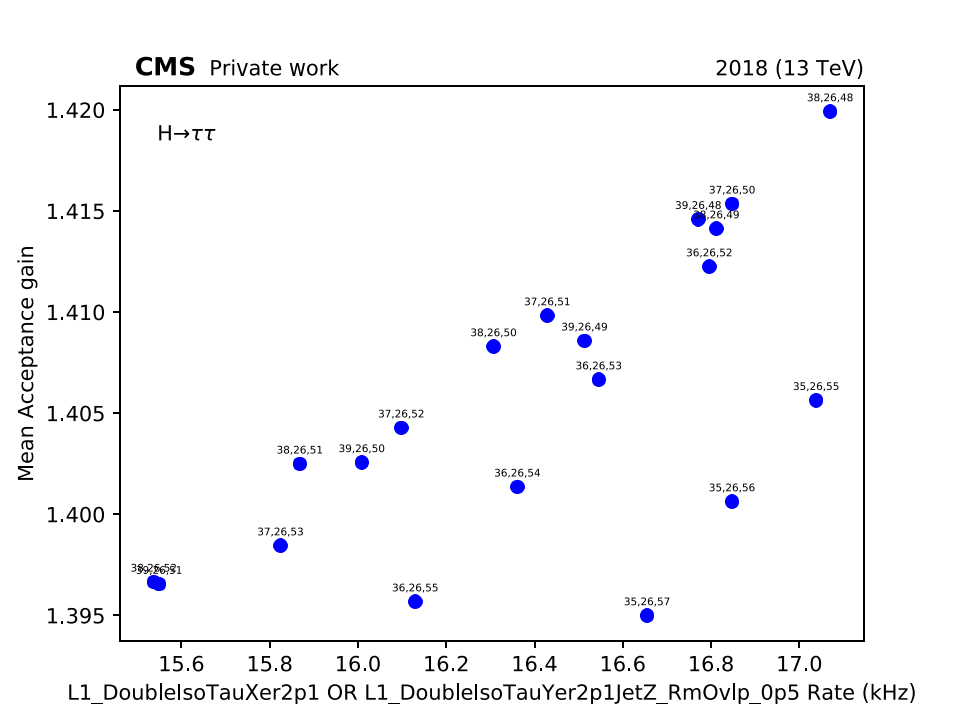
\includegraphics[width=0.49\textwidth]{Images/rate_vs_mean_acceptance__min5.0___max17.1___xx_sym__yy_sym_htt.pdf}}
\subfloat{\centering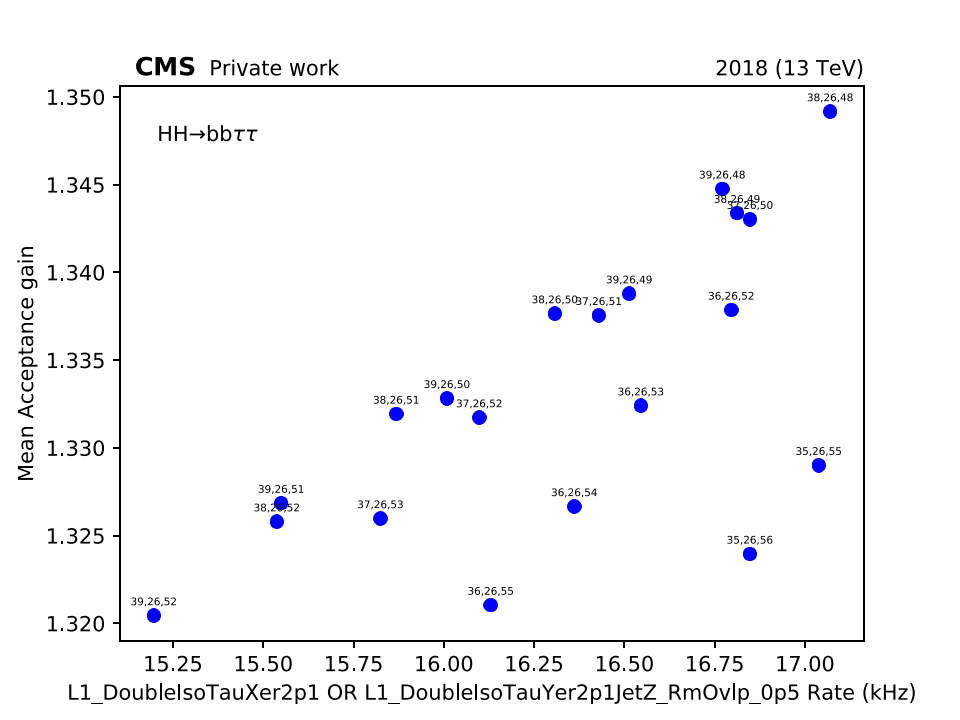
\includegraphics[width=0.49\textwidth]{Images/rate_vs_mean_acceptance__min5.0___max17.1___xx_sym__yy_sym_hhbbtt.pdf}}
\caption[Mean acceptance gains]{Mean acceptance gain for the H~$\to\tau\tau$ (left) and HH~$\to$~bb$\tau\tau$ (right) processes when considering the new trigger strategy for given $(X,Y,Z)$ $p_T$ thresh\-olds.}
\label{hh:fig:l1_trig_mean_acc}
\end{figure}

\begin{table}[h!]
\begin{small}
\begin{center}
\begin{tabular}{|l|r|r|r|}
\hline
Trigger seed & \multicolumn{2}{c|}{Acceptance gain} &  Rate (kHz) \\
\hline\hline
& H~$\to\tau\tau$ & HH~$\to$~bb$\tau\tau$ &  \\\hline
\texttt{L1\_DoubleIsoTau26er2p1\_Jet55\_RmOvlp\_dR0p5} & 44$\%$ & 36$\%$& $8.3 \pm 2.8$ \\
\texttt{L1\_DoubleIsoTau26er2p1\_Jet70\_RmOvlp\_dR0p5} & 34$\%$ & 29$\%$ & $5.3 \pm 1.8$ \\\hline
\end{tabular}
\end{center}
\end{small}

\caption[Rates and mean acceptance gains for the two new double-$\tau_h$+jet seeds]{Rates and mean acceptance gains for the two new double-$\tau_h$+jet seeds.}
\label{hh:tab:l1trig:allseeds}
\end{table}

%\begin{tabular}{|l|r|rr|rr|rr|r|}
%\hline
%\multicolumn{2}{|r|}{} & \multicolumn{2}{r|}{$H\to\tau\tau$, 1-jet, high $p_T$ cat.} & \multicolumn{2}{r|}{$H\to\tau\tau$, 2-jet cat.} & \multicolumn{2}{r|}{ $HH\to bb\tau\tau$} & \\\hline
% Parameters   &   Rate &    ggH &   VBFH &   ggH &  VBFH &   ggHH &   VBFHH &   Mean \\
%\hline
% 32,26,55     &  18.03 &                           1.50 &                           1.49 &                    1.35 &                    1.43 &           1.29 &           1.42 &   1.41 \\
% 32,26,70     &  16.42 &                           1.37 &                           1.38 &                    1.27 &                    1.34 &           1.25 &           1.34 &   1.33 \\
% 35,26,55     &  15.34 &                           1.47 &                           1.47 &                    1.29 &                    1.39 &           1.27 &           1.39 &   1.38 \\
% 35,26,70     &  13.27 &                           1.31 &                           1.33 &                    1.18 &                    1.27 &           1.20 &           1.28 &   1.26 \\
%\hline
%\end{tabular}


\section{Performance of the L1 double-$\tau_h$ + jet trigger}
\label{hh:sec:l1_performance}

The LHC Run 3 started during summer 2022 with the first proton-proton collisions at $\sqrt{s}=13.6$~TeV. In general, 2450 bunches were allocated per beam, resulting in an average PU of around 50~GeV at the start of the fill.

Before the start of the LHC Run 3 (summer 2022), the new L1 double-\tauh{}+jet seed (and its backup seed) were included in the L1 menu, so they can be used in physics analyses. Being included in the menu also allowed to study their rate and performance directly using 2022 collision data, where te seeds were enabled, and validating the expected results obtained by emulating the new seeds on 2018 data. Note that the expected beam conditions have changed between those results and the actual data taking, so the predictions need to be slightly modified.

In the following, performance results will be shown for the main L1 trigger seed.

\subsubsection{Rate with 2022 data}

Fig.~\ref{hh:fig:l1_rate_run3} shows the rate obtained for the L1 double-\tauh{}+jet seed using a collision data sample taken during 2022 as a function of the average PU. Note how the rate scales almost linearly with respect to the PU. Regarding the 2018 estimations, by rescaling the $8.3\pm2.8$~kHz obtained with 2018 data for PU 53 and 2748 bunches to 2450 bunches, a value of $7.4\pm2.5$~kHz is obtained, which agrees with the values obtained with 2022 data.


\begin{figure}[h!]
\begin{center}
\includegraphics[width=0.6\textwidth]{Images/L1_rate}
\end{center}
\caption[\texttt{L1\_DoubleIsoTau26er2p1\_Jet55\_RmOvlp\_dR0p5} seed rate]{\texttt{L1\_DoubleIsoTau26er2p1\_Jet55\_RmOvlp\_dR0p5} seed rate as a function of the PU for a collision data sample collected during 2022. Outliers come from runs taken with smaller number of bunches.}
\label{hh:fig:l1_rate_run3}
\end{figure}

\subsubsection{Trigger efficiency}

In order to measure the performance of a trigger selection, a good estimator is the trigger efficiency. This efficiency is computed as the fraction of events satisfying some requirements on the offline and trigger objects of the event over the ones satisfying the offline requirements. In general, this efficiency is computed with respect to the offline quantities related to the objects used in the trigger selection. For instance, in the double-$\tau_h$+jet trigger, this efficiency will be measured with respect to some quantities related to a pair of $\tau_h$ and a jet. In a simple 1-D case, where the algorithm only depends on one variable from one object, the shape of the efficiency as a function of the corresponding offline variable is commonly known as a \textit{turn-on} curve, which is a convolution of an step function (changing from 0 to 1 in the threshold used in the online selection) and a Gaussian resolution function, which represents the difference in resolution between the trigger and offline reconstruction. The more similar the trigger and offline reconstruction, the sharper would be the turn-on curve.

The efficiency for the double-$\tau_h$+jet trigger can be obtained as the product of the efficiencies for each individual trigger object, i.e.
\begin{equation}
\label{hh:eq:eff_per_legs}
\text{efficiency}_{(\tau_1,\tau_2,\text{jet})} = \text{efficiency}_{\tau_1}\times\text{efficiency}_{\tau_2}\times\text{efficiency}_{\text{jet}},
\end{equation}
where the individual trigger objects should satisfy the same kinematic requirements as in the double-$\tau_h$+jet trigger. A caveat from this method is that the efficiencies for each object are being considered independent from the other objects, while a correlation between them could appear. This particularity will be studied in future analysis.


In order to measure the efficiency for each single object, a tag and probe technique (already presented in previous chapters) is considered. In this method, we profit of the production of a known resonance that decays into two particles: a \textit{tag} particle, which satisfy very tight identification and isolation requirements to ensure it comes from the decay of the resonance, and a \textit{probe} particle, which is compatible with the resonance and is used to measure the efficiency.

In the double-$\tau_h$ analysis, the $\tau_h$ efficiency will be measured by considering the production of a Z boson that decays into two $\tau_h$. One $\tau_h$ decays leptonically into a muon and two neutrinos; the other, hadronically. The muon from the first decay will be used for tagging, while the $\tau_h$ will be used for efficiency computation. The tau trigger efficiency will be measured using a newly developed monitoring seed coded as \texttt{L1\_Mu18er2p1\_Tau26er2p1}, a trigger that requires one muon with $p_T\geq18$~GeV and $|\eta|<2.1$, and a $\tau_h$ with $p_T\geq26$~GeV and $|\eta|<2.1$ (i.e. the same kinematic restrictions as the double-$\tau_h$+jet seed under study with the exception of the isolation cut). Thus, the $\tau_h$ efficiency will be obtained as
\begin{equation}
\text{efficiency} = \frac{N_\text{pass}}{N_\text{all}},
\end{equation}
where $N_\text{all}$ is the number of events firing a single muon L1 trigger (encoded as \texttt{L1\_SingleMu22}), where one muon and at least one $\tau_h$ were reconstructed and the muon is matched to the muon used for triggering. Several quality cuts are applied to the reconstructed muon ($p_T>24$~GeV, $|\eta|<2.1$), the reconstructed $\tau_h$ ($|\eta|<2.1$, $d_z<0.2$~cm, VVVLoose DeepTauVsmu, VVVLoose DeepTauVse and Medium DeepTauVsjet working points) and the $\mu\tau_h$ system ($\Delta R(\mu, \tau_h) > 0.5$, invariant mass between 30 and 80~GeV). $N_\text{pass}$ is the number of events out of $N_\text{all}$ where the offline $\tau_h$ was matched to a trigger-level $\tau_h$ associated to the monitoring seed \texttt{L1\_Mu18er2p1\_Tau26er2p1}. The trigger-level $\tau_h$ is required to be isolated in order to fully match the $\tau_h$ requirements in the double-$\tau_h$+jet seed. 

When computing the efficiency for a given trigger with a tag and probe method, the samples used for this calculation need to be unbiased at trigger level, i.e. the events in the sample must not be selected by any trigger that targets the probe object. CMS stores in a particular data set all events that fired a muon-related trigger. Therefore, without any bias, we can use this data set to obtain the $\tau_h$ and jet trigger efficiencies using real collision data, and then obtain the efficiency for the double-$\tau_h$+jet trigger seed. The efficiency will also be computed with a Z + 2 jets simulated sample, so a comparison between the performance in real data and simulation can be obtained. Fig.~\ref{hh:fig:l1_eff_tauleg} shows the $\tau_h$ efficiency with respect to the offline $\tau_h$ $p_T$ and $\eta$ for the data and simulated sample.






\begin{figure}[h!]
\begin{center}
\subfloat{\includegraphics[width=0.49\textwidth]{Images/L1_ditaujet_tauleg_pt}}
\subfloat{\includegraphics[width=0.49\textwidth]{Images/L1_ditaujet_tauleg_eta}}
\end{center}
\caption[L1 $\tau_h$ trigger efficiency]{L1 $\tau_h$ trigger efficiency obtained with a tag and probe method with respect to the offline $\tau_h$ $p_T$ (left) and $\eta$ (right) for data events collected during 2022 (black) and simulated events from a Z~+~2 jets sample (red). Simulated events are reweighed so their PU distribution matches the one from the data (see Fig.~\ref{hh:fig:trig_pu_dist}). Generator-level weights are applied to the simulated events. Note that a $\tau$ $p_T>26$~GeV cut is imposed in the efficiency with respect to $\tau$ $\eta$ to match the $\tau$ $p_T$  threshold at trigger level.}
\label{hh:fig:l1_eff_tauleg}
\end{figure}

The trigger jet efficiency can be also computed in a similar way. In this case, $N_\text{all}$ includes all events firing the \texttt{L1\_Mu18er2p1\_Tau26er2p1} trigger, where one muon, at least one $\tau_h$, and at least one jet were reconstructed, and the muon and the $\tau_h$ are matched to the muon and the $\tau_h$ used for triggering. The previous quality cuts are applied for the muon and the $\tau_h$, while the jets are required to satisfy the tight particle-flow jet identification working point, $\Delta R(\mu, \text{jet}) > 0.5$, and $\Delta R(\tau_h, \text{jet}) > 0.5$. Out of these events, $N_\text{pass}$ are the ones where the offline jet matched a trigger jet associated to a newly developed monitoring seed encoded as \texttt{L1\_Mu18er2p1\_Tau26er2p1\_Jet55}. Fig.~\ref{hh:fig:l1_eff_jetleg} shows the jet efficiency with respect to the offline jet $p_T$ and $\eta$.

\begin{figure}[h!]
\begin{center}
\subfloat{\includegraphics[width=0.49\textwidth]{Images/L1_ditaujet_jetleg_pt}}
\subfloat{\includegraphics[width=0.49\textwidth]{Images/L1_ditaujet_jetleg_eta}}
\end{center}
\caption[L1 jet trigger efficiency]{L1 jet trigger efficiency obtained with a tag and probe method with respect to the offline jet $p_T$ (left) and $\eta$ (right) for data events collected during 2022 (black) and simulated events from a Z~+~2 jets sample (red). Simulated events are reweighed so their PU distribution matches the one from the data (see Fig.~\ref{hh:fig:trig_pu_dist}). Generator-level weights are applied to the simulated events. Note that a jet $p_T>55$~GeV cut is imposed in the efficiency with respect to jet $\eta$ to match the jet $p_T$  threshold at trigger level.}
\label{hh:fig:l1_eff_jetleg}
\end{figure}


\begin{figure}[h!]
\begin{center}
\includegraphics[width=0.6\textwidth]{Images/pu_dist}
\end{center}
\caption[PU distributions in 2022]{PU distribution for the data (black) and simulated (red) events used for the efficiency computation.}
\label{hh:fig:trig_pu_dist}
\end{figure}



\section{The HLT double-$\tau_h$ + jet path}
\label{hh:sec:hlt_doubletaujet}

In order to trigger on double-$\tau_h$ + jet events, an HLT path was designed and implemented, associated to the main L1 seed described in Section~\ref{hh:sec:l1seeds}. Additionally, a backup HLT path was also implemented triggered by the backup L1 seed. The structure of these paths is shown in Fig.~\ref{hh:fig:hlt_path}. This structure is very similar to the existing double-\tauh{} paths in Runs 1 and 2, but with some improvements developed for Run 3.

\begin{figure}
\begin{center}
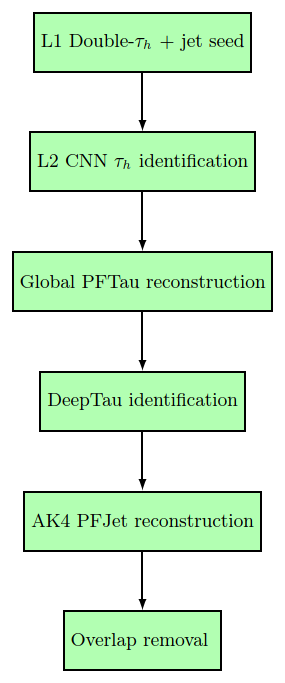
\includegraphics[width=0.4\textwidth]{Images/HLT_Path}
\end{center}
\caption[HLT path structure]{Sketch of the structure followed by the implemented HLT double-$\tau_h$ + jet path.}
\label{hh:fig:hlt_path}
\end{figure}

For an event to pass the HLT path, the first requirement is to pass the L1 seed requirements. On top of these L1 requirements, a typical HLT di-$\tau_h$ requirement is applied \cite{intro:exp:cms_trigger}: each L1 tau is used to build a Level-2 (L2) $\tau$ by associating the L1 tau all objects that fall into a $\Delta R$ cone of 0.5 with respect to it. Then, a filter is added based on a Convolutional Neural Network (CNN), aimed to reduce the number of background objects entering the next steps of the path (more time consuming) while reducing the least possible the number of true $\tau$ filtered. This machine learning approach is one of the new additions to Run 3 $\tau$ paths, resulting in an increase of efficiency and a decrease of rate with respect to the approaches used in the previous data-taking periods. 

After building the L2 $\tau$, global PF $\tau$ are reconstructed, similarly as how it was shown in Section~\ref{intro:subsec:taus}. PF $\tau$ are then filtered based on the same \deeptau{} algorithm as in the offline reconstruction level. This is another improvement introduced during Run 3, resulting in better signal purity and rate reduction.

At each step, at least a pair of $\tau$ leptons needs to survive the selection. Also, the two finally selected $\tau_h$ need to match the L1 $\tau$ used for triggering at L1 within a $\Delta R$ of 0.5, and their $p_T$ must be higher than 30~GeV.

After selecting the two $\tau_h$, the PF algorithm is used again to reconstruct the PF jets in the event. These PF jets will be selected if they satisfy an overlap removal criteria similar to the one used at L1: no matching (within a $\Delta R$ cone of 0.5) between the jet and a pair of PF $\tau$ that passed the whole HLT selection. On top of this criteria, the jet must match a L1 jet used for triggering and have a $p_T$ higher than a given threshold. For the main HLT path (triggered with the L1 seed with the 55~GeV jet $p_T$ threshold), this threshold is set to 60 GeV, while for the backup path, it is set to 75 GeV.

All these selections are grouped into two HLT paths, a main path and a backup path, encoded as \texttt{HLT\_Double\-MediumDeepTauPFTau30\_L2NN\_eta2p1\_PFJet60} and\\\texttt{HLT\-\_Double\-MediumDeepTau\-PF\-Tau30\-\_L2NN\_eta2p1\_PFJet75}, respectively.

\section{Performance of the double-$\tau_h$ + jet HLT path}
\label{hh:sec:hlt_performance}

\subsubsection{Expected rate using 2018 data}

To compute the expected rate from the new path, a similar approach to the one used in Section~\ref{hh:sec:l1seeds} is considered. The rate is estimated from a zero bias data sample taken during several 2018 runs corrected with the expected at that time Run-3 conditions (PU linearly scaled to 53 and 2748 colliding bunches). The rate obtained for this path is around $15.7\pm3.8$~Hz. Note that, as the expected rate by an HLT path is very small (around two to three orders of magnitude smaller than the correspondent L1 seed), a lot of zero bias events are needed to obtain a reasonably accurate result. In fact, even with all the 2018 runs that were used to obtain this value, only 15 events were able to pass the trigger, so the statistical uncertainty drives the result obtained.

For the sake of validating this result, the rate for the main L1 seed (\texttt{L1\_Double\-IsoTau26er2p1\_Jet55\_RmOvlp\_dR0p5}) described in Section~\ref{hh:sec:l1seeds} was also obtained in the same sample. The resulting value was 8.94~kHz, in agreement with the value obtained in the previous section. 

\subsubsection{Rate using 2022 data}

In parallel to the inclusion of the new L1 double-\tauh{}+jet seed (and its backup seed) in the L1 menu, their corresponding HLT paths were also included in the HLT menu. Fig.~\ref{hh:fig:hlt_rate_run3} shows the rate distribution for the HLT double-\tauh{}+jet path obtained from the same collision data sample used for the L1 seed rate estimation. In this case, the rate scaling with respect to PU is not as linear as for the L1 seed. However, for PU 53 we obtain a rate of around 15~Hz, in agreement with our expectation using 2018 data (after rescaling it by the number of bunches).

\begin{figure}[h!]
\begin{center}
\includegraphics[width=0.6\textwidth]{Images/HLT_rate}
\end{center}
\caption[\texttt{HLT\_Double\-MediumDeepTauPFTau30\_L2NN\_eta2p1\_PFJet60} path rate]{\texttt{HLT\_Double\-MediumDeepTauPFTau30\_L2NN\_eta2p1\_PFJet60} path rate as a function of the PU for a Run 3 collision data sample collected during 2022.  Outliers come from runs taken with smaller number of bunches.}
\label{hh:fig:hlt_rate_run3}
\end{figure}

\subsubsection{Total trigger efficiency}

In order for a trigger path to be used in the different analyses, the total trigger efficiency (i.e. the efficiency of firing both the HLT path and its corresponding L1 seed) has to be computed for both data and simulated events, so the latter can be reweighed by applying adequate scale factors. The procedure to obtain this efficiency is similar to the one shown for the L1 seeds: assuming the $\tau_h$ and jet objects are uncorrelated, the total efficiency can be computed as the product of the efficiency of selecting the leading $\tau$, the subleading $\tau$ and the jet.

The $\tau_h$ trigger efficiency can be measured through a tag-and-probe technique, as was done to compute the L1 efficiency, by selecting events that were triggered by a single-muon HLT path. Out of these events, the efficiency will be measured from the ones that also passed a HLT cross-trigger that requires a muon (used as tag) and a $\tau_h$ (used as probe). This path was implemented so that the selections applied on the muon are the same as in the single-muon path and the ones applied on the $\tau_h$ are the same requirements than in the double-$\tau_h$+jet path. Fig.~\ref{hh:fig:hlt_eff_tau} shows the efficiency as a function of the $\tau_h$ $p_T$ and $\eta$ for real data collected during Run 3 and simulated events from the previous Z~+~2 jets sample. 
Some differences can be seen between both samples, but will be corrected by including an scale factor for the simulated events.

\begin{figure}[h!]
\begin{center}
\subfloat{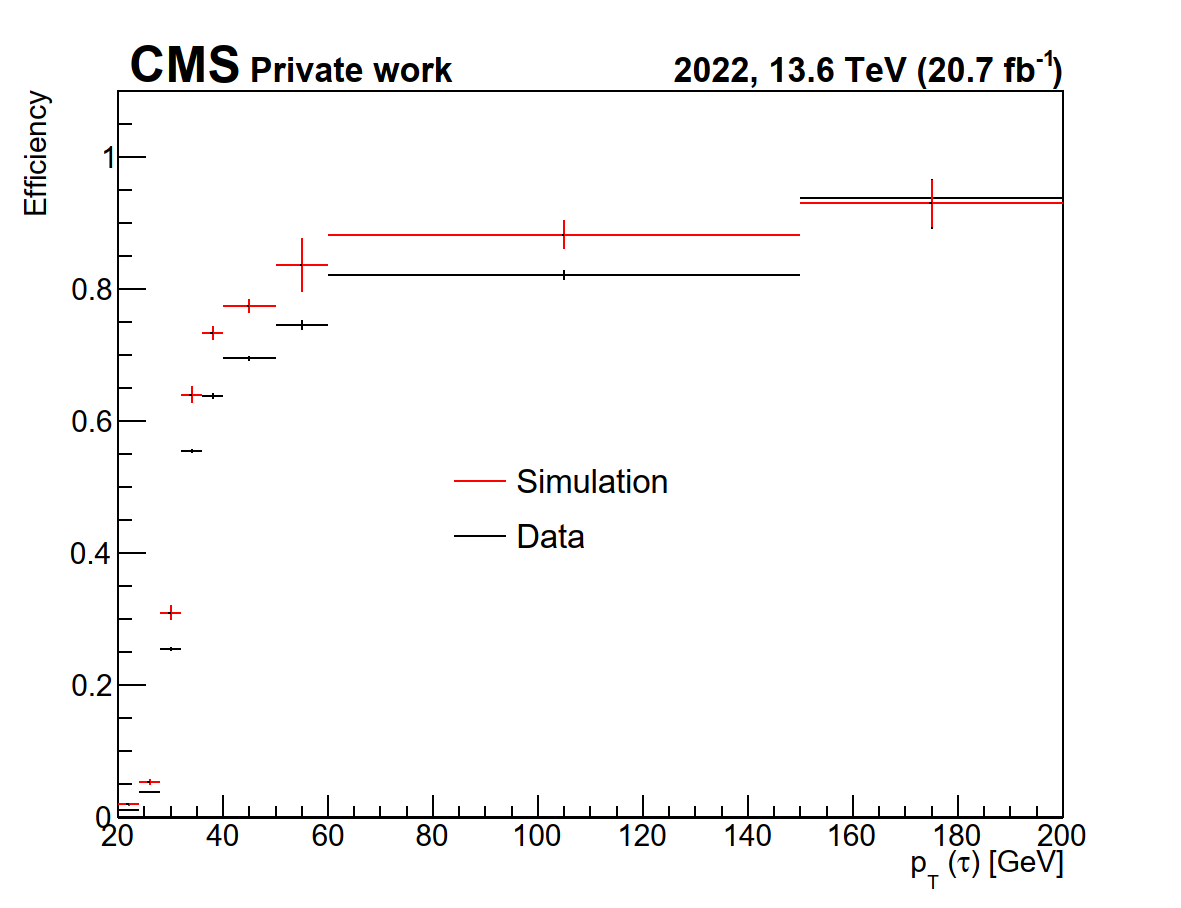
\includegraphics[width=0.49\textwidth]{Images/ditaujet_tauleg_pt}}
\subfloat{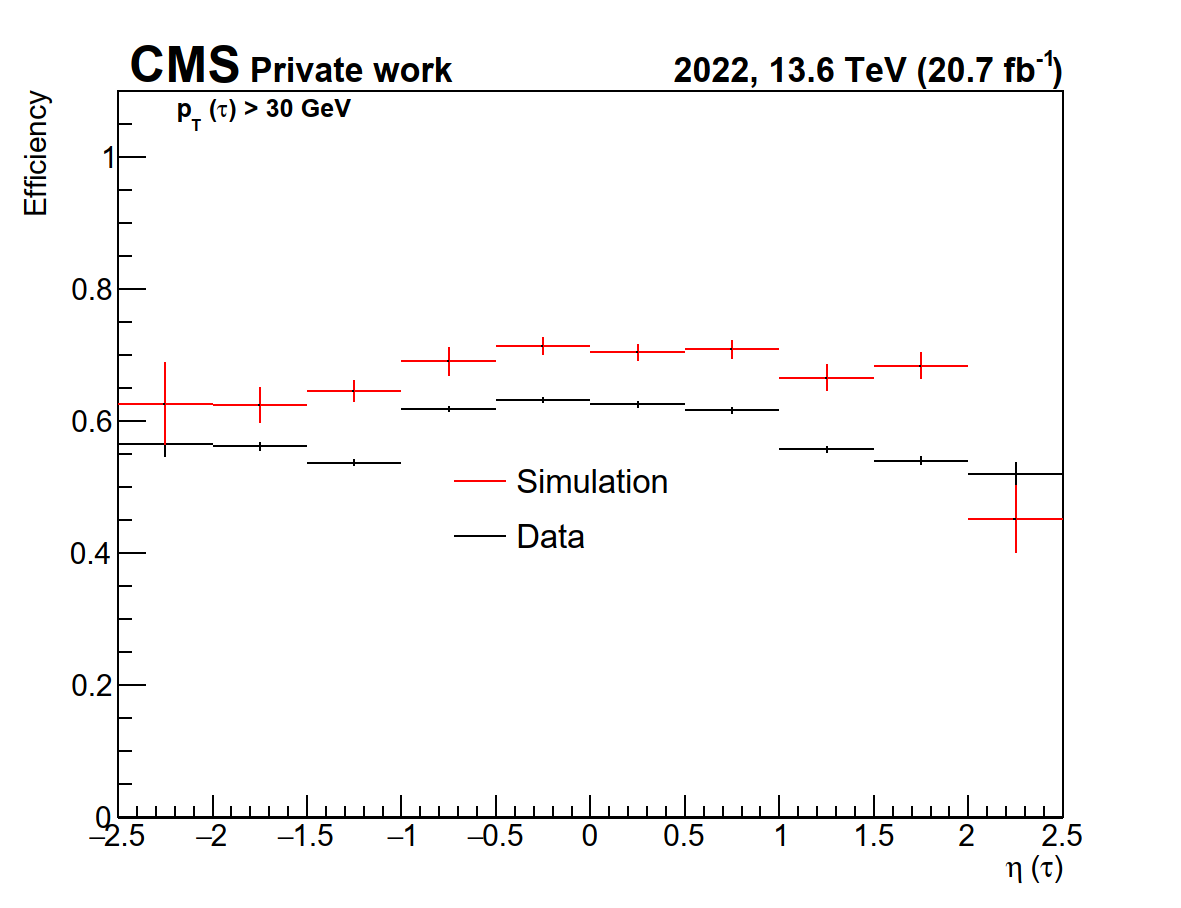
\includegraphics[width=0.49\textwidth]{Images/ditaujet_tauleg_eta}}
\end{center}
\caption[HLT $\tau_h$ trigger efficiency]{HLT $\tau_h$ trigger efficiency with respect to the offline $\tau_h$ $p_T$ (left) and $\eta$ (right) for data events collected during 2022 (black) and simulated events from a Z~+~2 jets sample (red). Simulated events are reweighed so their PU distribution matches the one from the data (see Fig.~\ref{hh:fig:trig_pu_dist}). Generator-level weights are applied to the simulated events.  Note that a $\tau$ $p_T>30$~GeV cut is imposed in the efficiency with respect to $\tau$ $\eta$ to match the $\tau$ $p_T$ threshold at trigger level.}
\label{hh:fig:hlt_eff_tau}
\end{figure}

In a similar way, the jet trigger efficiency is measured by selecting events with one muon, at least one $\tau_h$ and at least one jet that were triggered by the muon-$\tau_h$ cross-trigger. Out of these events, the efficiency will be computed from the ones that were triggered by an HLT muon-$\tau_h$-jet cross trigger, where the requirements on the trigger muon and $\tau_h$ are the same as in the muon-$\tau_h$ cross trigger and the requirements on the jet are the same as in the double-$\tau_h$+jet trigger. Fig.~\ref{hh:fig:hlt_eff_jet} shows the efficiency as a function of the jet $p_T$ and $\eta$ for real data collected during Run 3 and simulated events from the previous Z~+~2 jets sample. The agreement between data and simulated events is even better than for the $\tau_h$, although some disagreement is appreciated mostly in the energy range where the turn-on is produced.

\begin{figure}[h!]
\begin{center}
\subfloat{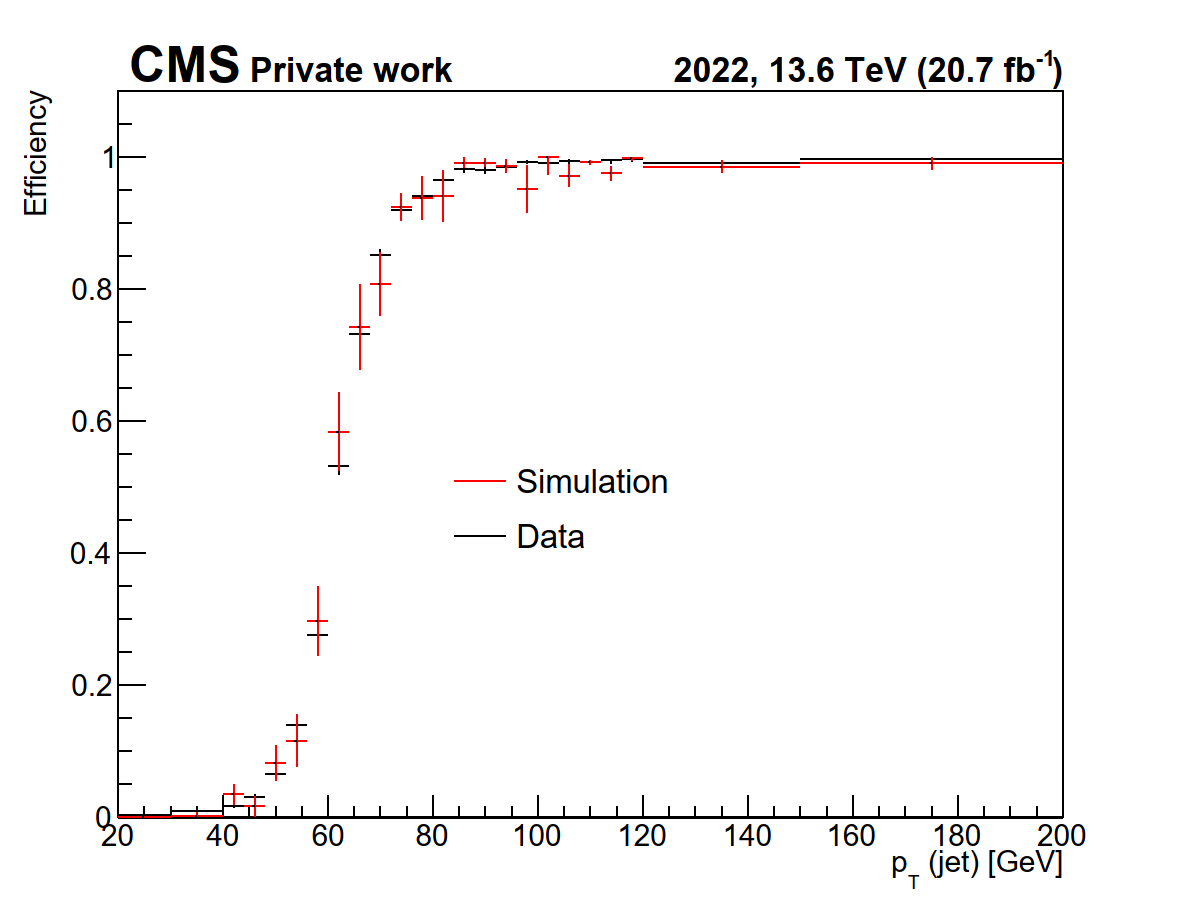
\includegraphics[width=0.49\textwidth]{Images/ditaujet_jetleg_pt}}
\subfloat{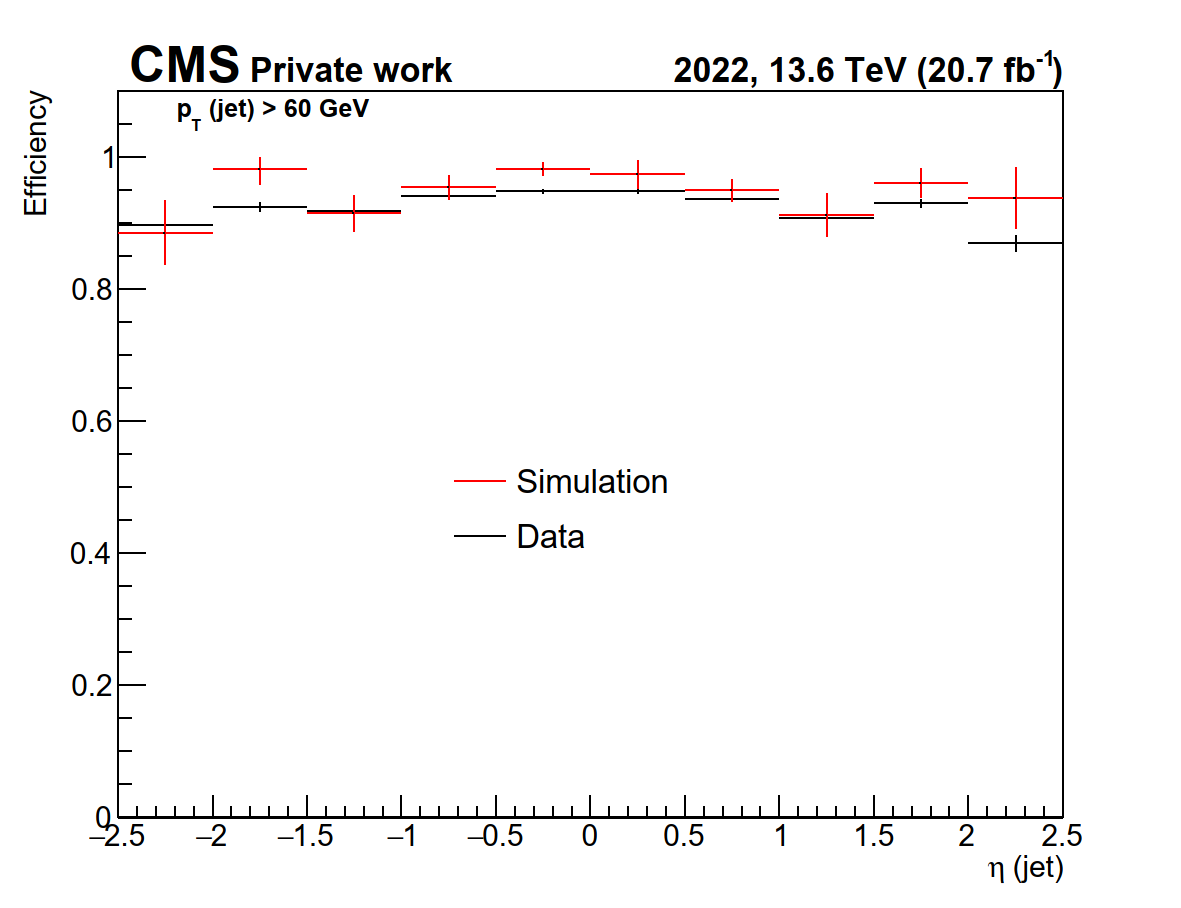
\includegraphics[width=0.49\textwidth]{Images/ditaujet_jetleg_eta}}
\end{center}
\caption[HLT jet trigger efficiency]{HLT jet trigger efficiency with respect to the offline jet $p_T$ (left) and $\eta$ (right) for data events collected during 2022 (black) and simulated events from a Z~+~2 jets sample (red). Simulated events are reweighed so their PU distribution matches the one from the data (see Fig.~\ref{hh:fig:trig_pu_dist}). Generator-level weights are applied to the simulated events.  Note that a jet $p_T>60$~GeV cut is imposed in the efficiency with respect to jet $\eta$ to match the jet $p_T$ threshold at trigger level.}
\label{hh:fig:hlt_eff_jet}
\end{figure}


%\bibliographystyle{plain}
%\bibliography{../biblio.bib}

\subsubsection{Expected sensitivity with Run 3 simulation}

A different test that can be performed, more close to analysis level, is to try to estimate the sensitivity gain when considering both the double-\tauh{} and double-\tauh{}+jet triggers instead of only considering the double-\tauh{} trigger, as done in the Run 2 \hhbbtt{} analysis. Four different samples generated for Run 3 analysis are considered, two signals (SM \hhbbtt{} produced via ggF and VBF) and two of the main backgrounds (inclusive \ttbar{} and the previous Z~+~2 jets sample). Over these samples, we apply the selection described in Sec.~\ref{hh:subsec:htt_pair_selection} in order to select the two $\tau$ coming from one of the Higgs bosons in the \hhbbtt{} analysis. In the \tauh\tauh{} channel, two trigger strategies will be considered. The first one consists of selecting only the events that fired the double-$\tau_h$ trigger with a 35~GeV $p_T$ threshold. This trigger was updated before Run 3, so it includes the new features also added to the double-$\tau_h$+jet trigger. In this case, the selected $\tau_h$ are required to have a $p_T>40$~GeV, as done in the \hhbbtt{} analysis. On the other hand, the second strategy consists of selecting events triggered by the double-$\tau_h$ or the new double-$\tau_h$+jet triggers. As the double-$\tau_h$+jet trigger requires two $\tau_h$ with $p_T>30$~GeV, the offline requirement can be lowered to 35~GeV. This way, more events could satisfy the lepton pair selection and be used for the signal extraction.  Additionally, for events trigged by the double-$\tau_h$+jet path, an offline jet with $p_T>65$~GeV is required.

Table~\ref{hh:tab:doubletaujet_sensitivity} shows the event yields for the four samples and the two trigger strategies for a given luminosity of 38~fb${}^{-1}$ (approximately the collected by CMS during 2022). An increase in the amount of signal events collected with the two triggers of 15\% and 19\% can be seen for the HH ggF and HH VBF samples, respectively. With the obtained event yields for both signals and backgrounds, the relative increase of significance can be computed as
\begin{equation}
\Delta S = \frac{\left(\frac{N(S)}{\sqrt{\sum_i N(B_i)}}\right)_{2\tau_h \text{ OR } 2\tau_h+j}}{\left(\frac{N(S)}{\sqrt{\sum_i N(B_i)}}\right)_{2\tau_h}},
\end{equation}
where $N(S)$ is the signal event yield, $N(B_i)$ is the event yield for a background $i$, and OR is the logical function OR between the two triggers. The relative increase of significance for the ggF sample takes a value of 6\%, while for the VBF sample, a 9\% value is obtained.


\begin{table}[h!]
\begin{small}
\begin{center}
\begin{tabular}{c | c c c c}
                                                                             & HH ggF & HH VBF & \ttbar{} & Z + 2 jets \\\hline
Double-\tauh{} trigger                                                        & 43.03   & 1.57   & 23440 & 94499      \\
Double-\tauh{} OR double-\tauh{}+jets triggers                                & 49.25   & 1.84   & 28530  & 108501      \\
Double-\tauh{} OR double-\tauh{}+jets / Double-\tauh{}                        & 1.14   & 1.18   & 1.22  & 1.15      

\end{tabular}
\end{center}
\end{small}

\caption[Sensitivity increase with the new trigger strategy]{Expected event yields in the \tauh\tauh{} channel after the \hhbbtt{} $\tau\tau$ pair selection for HH ggF, HH VBF, \ttbar{} and Z~+~2 jets for two different trigger strategies, considering only the double-\tauh{} trigger or both the double-\tauh{} and the double-\tauh{}+jet triggers. The third row of the table is the event ratio between the two trigger strategies. An integrated luminosity of 38~fb${}^{-1}$ (approximately the collected during 2022) has been considered.}
\label{hh:tab:doubletaujet_sensitivity}
\end{table}

\section{Summary}

In view of the new LHC data taking period (Run 3, 2022-2025), a new trigger strategy for the \htt{} and \hhbbtt{} analyses has been studied, focusing on the fully-hadronic $\tau$ pair decay mode (\tauh\tauh{}). This new strategy consists of including in the L1 and HLT menus a trigger that requires two \tauh{} and one jet, where the $p_T$ threshold on the \tauh{} is smaller than the one present in the double-\tauh{} trigger, already available in the Run 2 menus. By lowering this $p_T$ threshold, more \tauh{} would be available for triggering and the acceptance on the \htt{} and \hhbbtt{} analyses would increase.

Regarding the L1 seed, a complete process was performed in order to obtain the optimal $p_T$ thresholds to be used for both \tauh{} and jet in the seed. This optimization was based on having a compromise between the acceptance gained and the rate added. The optimization process lead to adding two new double-\tauh{}+jet seeds to the L1 menu: a main seed, with a \tauh{} $p_T$ threshold of 26~GeV and a jet $p_T$ threshold of 55~GeV, and its backup seed, with $p_T$ thresholds of 26~GeV and 70~GeV for the \tauh{} and jet, respectively. By considering the main seed, an estimation of the acceptance increases in the \htt{} and \hhbbtt{} obtained values of 44\% and 36\%, respectively, while adding around 8~kHz total rate on a Run 2 sample adapted to the Run 3 data taking conditions.

The new L1 seeds were included in the L1 menu before the start of the LHC Run 3 (summer 2022), so they can be used in physics analyses. The rate and efficiency of the main L1 seed have been studied using 2022 collision data. The rate values obtained agree with the 2018 extrapolations. The trigger efficiency for both \tauh{} and jet objects has also been obtained with tag and probe techniques for both 2022 collision data and a Z + 2 jets simulated sample, achieving a good agreement between the two samples.

Once the L1 seed was implemented, its corresponding HLT path was also developed based on the existing double-\tauh{} path, already present in the Run 3 menu. This path includes new features developed for Run 3, such as a CNN for Level-2 $\tau$ filtering or the DeepTau algorithm for Particle Flow $\tau$ identification at trigger level. The rate of the Double-\tauh{}+jet path was estimated using 2018 data with Run-3 conditions, obtaining around 16~Hz. The rate computed with 2022 collision data agrees with the expectations. The efficiency of both \tauh{} and jet objects has also been computed with 2022 collision data and the Z + 2 jets simulated sample. A very good agreement is achieved between the two samples.

Finally, a first test has been performed to compute an estimation of the sensitivity gain in the \hhbbtt{} analysis when considering the new trigger strategy: instead of just considering the double-\tauh{} trigger (as was done in the Run 2 analysis), computing the logical OR of this trigger and the new double-\tauh{}+jet trigger. When applying the $\tau\tau${} pair selection (both at trigger and offline level) and a minimal jet requirement if the event satisfied the double-\tauh{}+jet trigger selection, 6\% and 9\% sensitivity gains were obtained for the HH ggF and HH VBF samples, respectively.


\end{document}

